% American Journal of Physics submission manuscript — REVTeX 4.2.
% Double-spaced single-column review copy. For the typeset two-column journal
% look, change "preprint" -> "reprint" and comment out \doublespacing.
\documentclass[aip,preprint,amsmath,amssymb,floatfix]{revtex4-2}

\usepackage{graphicx}
\usepackage{booktabs}
\usepackage{setspace}
\usepackage{hyperref}

\doublespacing

\begin{document}

\title{A MemComputing Approach to Orbital Mechanics}

\author{Dietmar Henrich}
\affiliation{Chair of Materials Science and Nanotechnology,
Technische Universit\"{a}t Dresden, 01062 Dresden, Germany}

\author{Massimiliano Di Ventra}
\affiliation{Department of Physics, University of California San Diego,
La Jolla, CA 92093, USA}

\begin{abstract}
The MemComputing paradigm of computation employs time non-locality (memory) to
solve a given problem by mapping its solutions into fixed points of a dynamical
system. The problem is then solved not in the original state space of variables,
but in an augmented phase space of relaxed original variables plus memory degrees
of freedom. Although such an approach has been primarily used to solve
combinatorial optimization problems, here we show that it can be employed in the
field of celestial mechanics. As an important example we introduce a MemComputing
machine that discovers all five Lagrange equilibrium points of any restricted
three-body system in the solar system without prior knowledge of their location.
The dynamical system follows equations of motion in the co-rotating frame with a
dissipative term dynamically modified by a memory degree of freedom according to
the gradient of the Jacobi effective potential. We finally discuss the advantages
of this approach compared to existing methods.
\end{abstract}

\maketitle

%=============================================================================
\section{Introduction and scope}\label{sec:intro}
%=============================================================================

MemComputing is a non-von-Neumann paradigm in which a physical system exploits
\emph{time non-locality}---the ability of internal degrees of freedom to retain
and use information about their past state---to solve a
problem~\cite{diventra2022}. In a Digital MemComputing Machine (DMM) the memory
variables act as dynamic Lagrange multipliers: the solutions of the target
problem are mapped onto the stable fixed points of a continuous dynamical system,
so that trajectories launched from generic initial conditions are guided to a
solution along instanton paths~\cite{traversa2015,diventra2018}. The computation
proceeds in an augmented phase space whose coordinates are the relaxed original
variables \emph{plus} the memory degrees of freedom. To date this paradigm has
been applied mostly to combinatorial optimization (satisfiability, MaxSAT, prime
factorization)~\cite{traversa2017}. Here we show that it transfers naturally to a
continuous problem of celestial mechanics.

The restricted three-body problem (RTBP)---two massive primaries on a circular
orbit and a massless test particle---is a cornerstone of nonlinear dynamics and
of practical mission design~\cite{szebehely1967}. Its five equilibria, the
Lagrange points~\cite{lagrange1772}, are normally located by analytic or
numerical root finding that requires a separate bracket or initial guess for each
point and prior knowledge of the solution structure. We construct instead a
single MemComputing machine---an autonomous dynamical system in the co-rotating
frame whose dissipation is dynamically controlled by one memory degree of
freedom---that discovers all five Lagrange points of \emph{any} restricted
three-body system in the solar system from a generic grid of starting positions,
without being given the coordinates of any solution. We verify it on all
twenty-three Sun--planet and planet--moon pairs, spanning mass ratios from
$\mu \approx 2\times10^{-9}$ to $\mu \approx 0.1$, list every parameter needed to
reproduce the results, and close by comparing the approach with existing methods.

%=============================================================================
\section{The restricted three-body problem}\label{sec:rtbp}
%=============================================================================

We use the co-rotating frame in normalized units: the two primaries are separated
by unit distance, the orbital angular velocity of the frame is $\omega=1$, and the
mass ratio is
\begin{equation}
  \mu = \frac{M_2}{M_1+M_2}\in(0,\tfrac12],
\end{equation}
placing the primary $M_1$ at $(-\mu,0)$ and the secondary $M_2$ at $(1-\mu,0)$.
The Jacobi effective potential is
\begin{equation}
  \Omega(x,y)=\frac{x^2+y^2}{2}+\frac{1-\mu}{r_1}+\frac{\mu}{r_2},
  \label{eq:omega}
\end{equation}
with $r_1=\sqrt{(x+\mu)^2+y^2}$ and $r_2=\sqrt{(x-1+\mu)^2+y^2}$; the first term
is the centrifugal potential of the rotating frame and the other two are the
gravitational wells of the primaries. Its gradient is
\begin{align}
  \partial_x\Omega &= x-\frac{(1-\mu)(x+\mu)}{r_1^3}-\frac{\mu(x-1+\mu)}{r_2^3},
  \label{eq:gx}\\
  \partial_y\Omega &= y-\frac{(1-\mu)\,y}{r_1^3}-\frac{\mu\,y}{r_2^3}.
  \label{eq:gy}
\end{align}
A Lagrange point is a relative equilibrium: in the rotating frame the test
particle is stationary, so all velocities and accelerations vanish and the
equilibrium condition reduces to the single vector clause
\begin{equation}
  \boxed{\;\nabla\Omega(x,y)=\mathbf 0\;}
  \label{eq:clause}
\end{equation}
which has exactly five solutions: the three collinear points $L_1,L_2,L_3$ on the
axis $y=0$ and the two triangular points
$L_{4,5}=(\tfrac12-\mu,\pm\tfrac{\sqrt3}{2})$~\cite{szebehely1967}.

A quantity central to the machine below is the transverse curvature of $\Omega$,
\begin{equation}
  \Omega_{yy}=1-\frac{1-\mu}{r_1^3}+\frac{3(1-\mu)y^2}{r_1^5}
              -\frac{\mu}{r_2^3}+\frac{3\mu y^2}{r_2^5}.
  \label{eq:oyy}
\end{equation}
On the axis $(y=0)$ it reduces to $1-(1-\mu)/r_1^3-\mu/r_2^3$, which is
\emph{negative} at all three collinear points (for Earth--Moon, $\mu=0.0121$:
$\Omega_{yy}=-4.15,-2.19,-0.011$ at $L_1,L_2,L_3$) and \emph{positive} ($+2.25$)
at $L_{4,5}$. Its sign therefore distinguishes the collinear saddle points from
the triangular extrema using only information available at the current position
(Fig.~\ref{fig:curv}).

\begin{figure*}[!t]
  \centering
  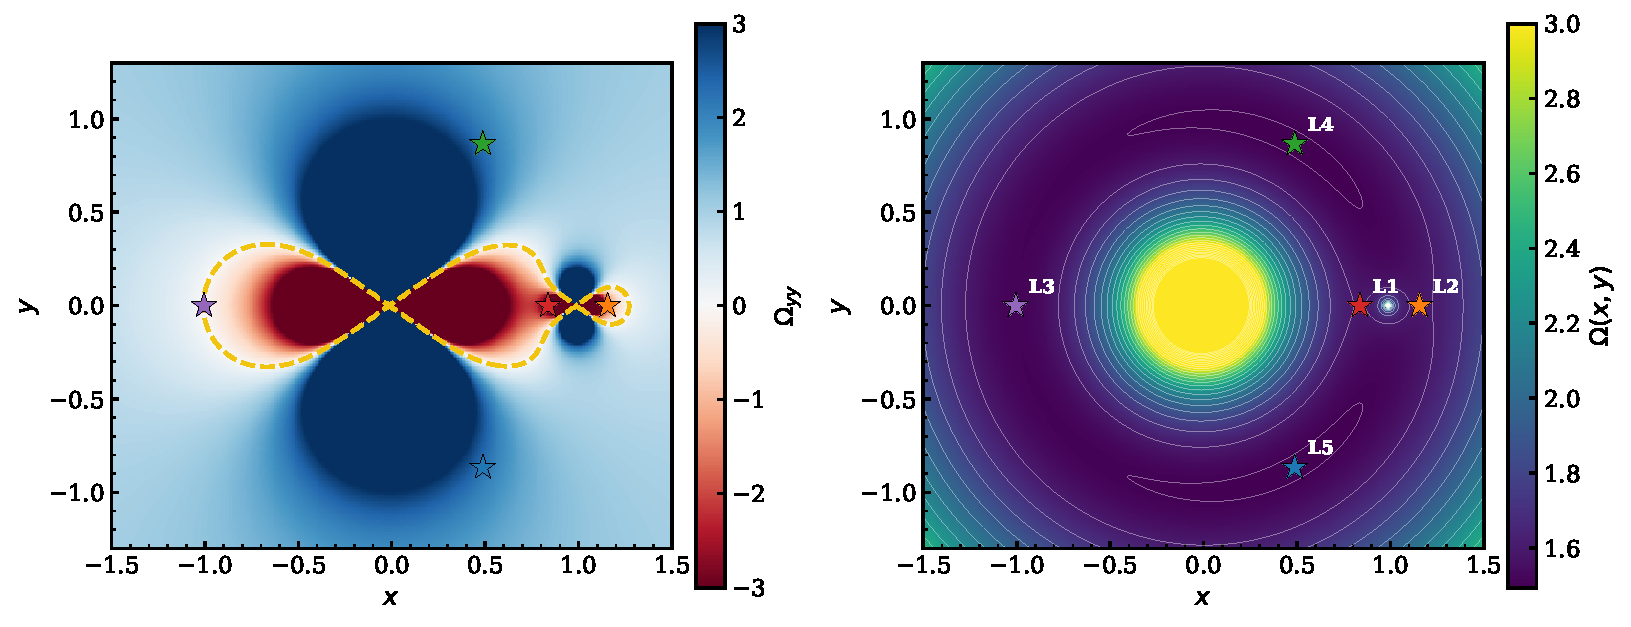
\includegraphics[width=0.92\textwidth]{fig_v3_curvature.pdf}
  \caption{%
    \textbf{Left}: the transverse curvature $\Omega_{yy}(x,y)$,
    Eq.~\eqref{eq:oyy}, for the Earth--Moon mass ratio (red--blue, clipped at
    $\pm3$); the dashed line is the contour $\Omega_{yy}=0$. Where $\Omega_{yy}<0$
    (red) the machine activates a correction current ($\sigma=+1$); elsewhere it
    descends normally ($\sigma=-1$). \textbf{Right}: the effective potential
    $\Omega(x,y)$, Eq.~\eqref{eq:omega}. Stars mark the five Lagrange points.}
  \label{fig:curv}
\end{figure*}

%=============================================================================
\section{The MemComputing machine}\label{sec:machine}
%=============================================================================

The machine is an autonomous dynamical system in the co-rotating frame. To the
ordinary rotating-frame equations of motion---the gradient force $-\nabla\Omega$
and the Coriolis acceleration---we add a viscous term whose coefficient is
\emph{not constant} but is set by a memory degree of freedom $m$:
\begin{subequations}\label{eq:dmm}
\begin{align}
  \ddot x &= 2\dot y - \partial_x\Omega - \gamma_{\rm eff}\,\dot x,
  \label{eq:vx}\\
  \ddot y &= -2\dot x + \sigma\,\partial_y\Omega - \gamma_{\rm eff}\,\dot y,
  \label{eq:vy}\\
  \dot m  &= \beta\,\lVert\nabla\Omega\rVert,\qquad m(0)=0,\quad m\le m_{\rm cap},
  \label{eq:mem}\\
  \gamma_{\rm eff} &= \gamma_0+\kappa\,m .
  \label{eq:geff}
\end{align}
\end{subequations}
The augmented phase space is $(x,y,\dot x,\dot y,m)$: the relaxed original
variables $(x,y)$ and their velocities, plus the single memory variable $m$.

\paragraph{Memory degree of freedom.}
Equation~\eqref{eq:mem} integrates the magnitude of the clause violation,
$\lVert\nabla\Omega\rVert$, so that
\begin{equation}
  m(t)=\beta\!\int_0^t\!\lVert\nabla\Omega(\mathbf r(\tau))\rVert\,d\tau .
  \label{eq:mint}
\end{equation}
Because the integrand is non-negative, $m$ is monotone non-decreasing: it ratchets
up while the clause $\nabla\Omega=\mathbf 0$ is unsatisfied and stops growing only
when $\lVert\nabla\Omega\rVert\to0$, i.e.\ exactly at a Lagrange point. Through
$\gamma_{\rm eff}=\gamma_0+\kappa m$ this accumulated history controls the
dissipation of the mechanical motion. The memory enters the dissipative channel
deliberately: the rate of change of the kinetic energy
$T=\tfrac12\lVert\dot{\mathbf r}\rVert^2$ along \eqref{eq:dmm} is
\begin{equation}
  \dot T = -\,\dot{\mathbf r}\!\cdot\!\nabla_{\!\sigma}\Omega
           \;-\;(\gamma_0+\kappa m)\,\lVert\dot{\mathbf r}\rVert^2 ,
  \label{eq:Tdot}
\end{equation}
where $\nabla_{\!\sigma}\Omega=(\partial_x\Omega,-\sigma\,\partial_y\Omega)$ and
the Coriolis force has dropped out because it does no work. The only
sign-definite, energy-removing term is the viscous one, and it is the memory $m$
that sets its strength. With $\gamma_0=0$ the memory is the \emph{sole} source of
dissipation: the flow is undamped at $t=0$ and acquires dissipation only as $m$
accumulates from the history of the clause violation. The monotone functional
\eqref{eq:mint} thus plays the role of a Lyapunov function, draining kinetic
energy until the trajectory is quenched at a fixed point of \eqref{eq:dmm}, which
by construction is a solution of the clause~\eqref{eq:clause}.

\paragraph{Curvature-adaptive correction current.}
At each step the machine evaluates the local curvature $\Omega_{yy}$,
Eq.~\eqref{eq:oyy}, and sets
\begin{equation}
  \sigma =
  \begin{cases}
    +1 & \Omega_{yy}<0 \quad(\text{correction current}),\\
    -1 & \Omega_{yy}\ge0 \quad(\text{ordinary descent}).
  \end{cases}
  \label{eq:sigma}
\end{equation}
At a collinear point a small transverse displacement $y>0$ gives
$\partial_y\Omega<0$ (because $\Omega_{yy}<0$), so the ordinary force
$-\partial_y\Omega>0$ would push the particle \emph{away} from the axis; setting
$\sigma=+1$ reverses it into a restoring force, turning the collinear saddle into
an attractor of the damped flow. Where $\Omega_{yy}>0$ the ordinary descent
already restores. The sign is read from the geometry at the current position; no
information about which equilibria are saddles is supplied. We use the full
gradient norm in Eq.~\eqref{eq:mem} (a single scalar memory) so that both axes are
damped equally; a per-axis memory would underdamp the transverse direction on the
collinear axis, where $|\partial_y\Omega|\approx0$, and the trajectory would drift
past $L_2,L_3$.

%=============================================================================
\section{Numerical implementation and parameters}\label{sec:params}
%=============================================================================

Everything below is the procedure actually integrated in the accompanying
code~\cite{github2026}; all parameters are collected in
Table~\ref{tab:params} so the results can be reproduced exactly.

\paragraph{Integration.}
Equations~\eqref{eq:dmm} are advanced with the explicit Euler method and a fixed
step $\Delta t$. A singularity guard $\varepsilon=10^{-9}$ is added to $r_1,r_2$.
A trajectory stops when $\lVert\nabla\Omega\rVert<\theta$ (the convergence
threshold), when it leaves the disk $\lVert\mathbf r\rVert>12$, or after
$N_{\max}$ steps.

\paragraph{Seed grid.}
No solution coordinates are given to the integrator. The starting positions are
generated from the \emph{generic structure} of the RTBP only---the rotating-frame
symmetry, the Hill scaling, and the equilateral configuration---using the Hill
radius $r_H=(\mu/3)^{1/3}$ and the secondary position $x_{\rm s}=1-\mu$:
\begin{itemize}
\item[(A)] \emph{on-axis seeds} $(x_{\rm s}\pm c\,r_H,\,0)$ for
  $c\in\{0.5,0.7,1.0,1.4,2.0,3.0,5.0,8.0\}$, which bracket the collinear $L_1,L_2$
  that lie within a Hill radius of the secondary on the axis $y=0$;
\item[(B)] \emph{$L_3$ seeds} at $(-1-5\mu/12,0)$, $(-0.96,0)$, $(-1.04,0)$,
  $(-1.10,0)$, opposite the primary;
\item[(C)] \emph{equilateral seeds} $(\tfrac12+\delta_x,\ \pm\tfrac{\sqrt3}{2}
  +\delta_y)$ for $\delta_x\in\{-0.12,-0.04,0.04,0.12\}$,
  $\delta_y\in\{-0.10,0,0.10\}$, around the triangular configuration;
\item[(D)] a coarse off-axis fill $(x,y)$ with $x\in\,$linspace$(-1.3,1.3,6)$ and
  $y\in\{\pm0.9,\pm0.45\}$, for the broad large-$\mu$ basins.
\end{itemize}
Seeds falling inside the exclusion disks around either primary---radius
$\varepsilon_1=\min(0.03,0.3\,r_H)$ about $M_1$ and
$\varepsilon_2=\min(0.012,0.3\,r_H)$ about $M_2$---are discarded. This yields of
order seventy starting positions per system. The seeds use no solution
coordinates: the collinear points are transcendental roots whose $\mu$-dependent
positions are not supplied, and even the equilateral seeds are placed at the
fixed point $(\tfrac12,\pm\tfrac{\sqrt3}{2})$ rather than the exact
$(\tfrac12-\mu,\pm\tfrac{\sqrt3}{2})$; the dynamics and the refinement below
produce the exact positions.

\paragraph{Refinement and labelling.}
Each stopped trajectory is optionally refined by a few Newton iterations on
$\nabla\Omega=\mathbf 0$ (using the analytic Hessian), accepted only if it
converges to a genuine zero, $\lVert\nabla\Omega\rVert<10^{-9}$, and otherwise
falling back to the raw endpoint. A converged point is identified with the
nearest of the five analytic Lagrange positions if it lies within $0.05$ (refined)
or $0.12$ (raw); these analytic positions are used only for post-hoc
identification and accuracy assessment, never by the integrator.

\begin{table}[ht]
\centering
\caption{Parameters used to produce all results. Control parameters are the same
for every system.}
\label{tab:params}
\begin{tabular}{lll}
\toprule
Symbol & Meaning & Value\\
\midrule
$\gamma_0$ & baseline damping & $0$\\
$\kappa$ & memory--damping gain & $1.0$\\
$\beta$ & memory growth rate & $0.5$\\
$m_{\rm cap}$ & memory cap & $10$\\
$\Delta t$ & Euler time step & $0.01$\\
$\theta$ & convergence threshold $\lVert\nabla\Omega\rVert$ & $10^{-4}$\\
$N_{\max}$ & maximum steps & $2\times10^{5}$\\
$\varepsilon$ & singularity guard on $r_1,r_2$ & $10^{-9}$\\
$\varepsilon_1$ & exclusion radius about $M_1$ & $\min(0.03,0.3\,r_H)$\\
$\varepsilon_2$ & exclusion radius about $M_2$ & $\min(0.012,0.3\,r_H)$\\
Newton xtol & refinement tolerance & $10^{-12}$\\
accept & refinement acceptance & $\lVert\nabla\Omega\rVert<10^{-9}$\\
\bottomrule
\end{tabular}
\end{table}

%=============================================================================
\section{Results}\label{sec:results}
%=============================================================================

Figure~\ref{fig:disc} shows representative trajectories of the machine for the
Earth--Moon system: each is an instanton path from a generic seed to one of the
five Lagrange points. Figure~\ref{fig:mem} tracks the internal dynamics along the
converging trajectories: the memory $m$ and the dissipation $\gamma_{\rm eff}=
\kappa m$ it generates ratchet upward from zero and saturate, the kinetic energy
$T$ is driven to zero, and the clause violation $\lVert\nabla\Omega\rVert$ decays
below threshold. The memory is doing the work: with $\gamma_0=0$ it is the only
term that removes energy.

\begin{figure}[!t]
  \centering
  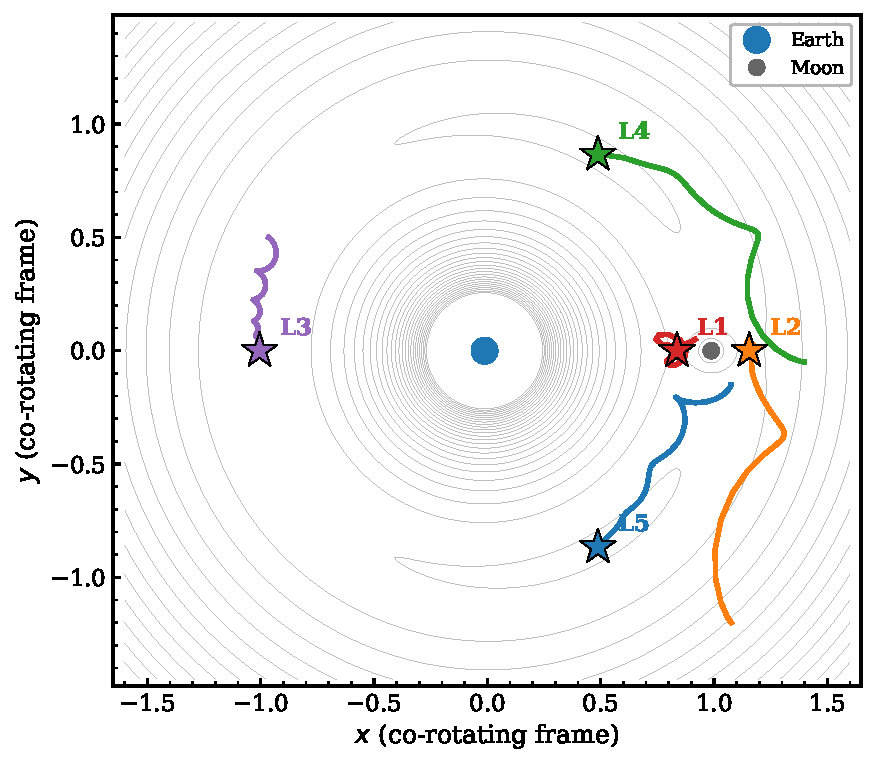
\includegraphics[width=0.99\columnwidth]{fig_v3_discovery.pdf}
  \caption{%
    Representative trajectories of the MemComputing machine for the Earth--Moon
    system ($\mu=0.0121$), one per Lagrange point. Grey curves: level sets of
    $\Omega$. Stars: the discovered equilibria. The integrator receives no
    solution coordinates.}
  \label{fig:disc}
\end{figure}

\begin{figure*}[!t]
  \centering
  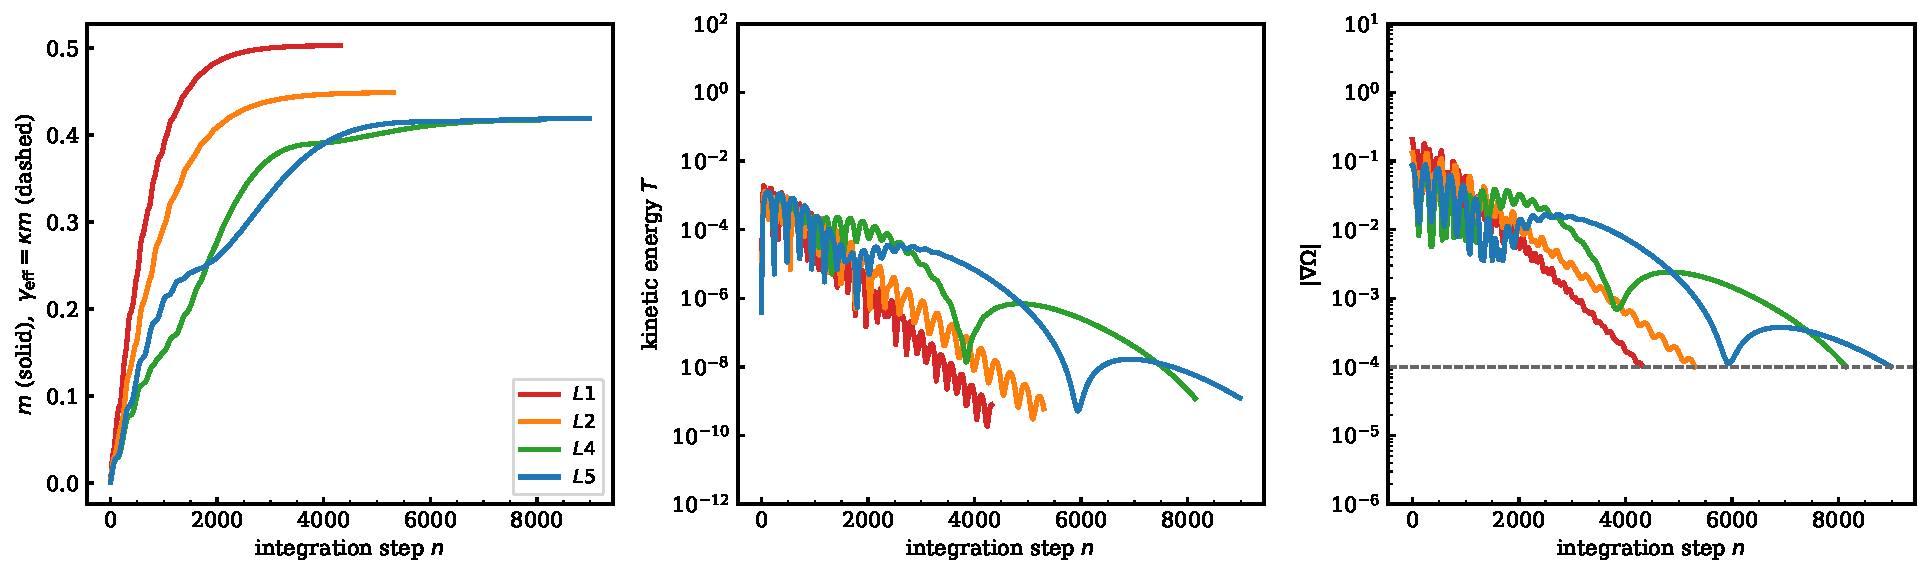
\includegraphics[width=0.98\textwidth]{fig_memory_clean.pdf}
  \caption{%
    Internal dynamics of the machine along the converging Earth--Moon
    trajectories. \textbf{Left}: memory $m$ (solid) and the dissipation it
    generates $\gamma_{\rm eff}=\kappa m$ (dashed) ratchet up and saturate.
    \textbf{Centre}: kinetic energy $T$ driven to zero (memory removes it).
    \textbf{Right}: clause violation $\lVert\nabla\Omega\rVert$ decays below the
    threshold $\theta=10^{-4}$ (dashed). Colour identifies the discovered
    L-point.}
  \label{fig:mem}
\end{figure*}

The central result is that the \emph{same} machine, with the \emph{same} control
parameters of Table~\ref{tab:params}, discovers all five Lagrange points of every
two-body system in the solar system. Table~\ref{tab:systems} lists the
twenty-three Sun--planet and planet--moon pairs, with mass ratios spanning eight
orders of magnitude, from Mars--Deimos ($\mu=2.3\times10^{-9}$) to Pluto--Charon
($\mu=0.11$). Every system returns $5/5$. After Newton refinement the located
positions agree with the analytic Lagrange points to better than $10^{-9}$. We
note that for $\mu<\mu_{\rm Routh}=0.03852$~\cite{routh1875} the triangular points
$L_4,L_5$ are linearly stable, satisfied by all systems except Pluto--Charon,
where the machine still locates them as solutions of $\nabla\Omega=\mathbf 0$.

\begin{table}[ht]
\centering
\caption{All five Lagrange points are found for every solar-system two-body pair,
using the single parameter set of Table~\ref{tab:params}. ``Stable'' refers to
the linear stability of $L_4,L_5$ (Routh, $\mu<0.03852$).}
\label{tab:systems}
\begin{tabular}{lccc}
\toprule
System & $\mu$ & Found & $L_4/L_5$ stable\\
\midrule
Mars--Deimos      & $2.3\times10^{-9}$ & $5/5$ & yes\\
Sun--Pluto        & $6.6\times10^{-9}$ & $5/5$ & yes\\
Mars--Phobos      & $1.7\times10^{-8}$ & $5/5$ & yes\\
Sun--Mercury      & $1.7\times10^{-7}$ & $5/5$ & yes\\
Saturn--Enceladus & $1.9\times10^{-7}$ & $5/5$ & yes\\
Sun--Mars         & $3.2\times10^{-7}$ & $5/5$ & yes\\
Sun--Venus        & $2.4\times10^{-6}$ & $5/5$ & yes\\
Sun--Earth        & $3.0\times10^{-6}$ & $5/5$ & yes\\
Saturn--Rhea      & $4.1\times10^{-6}$ & $5/5$ & yes\\
Jupiter--Europa   & $2.5\times10^{-5}$ & $5/5$ & yes\\
Uranus--Oberon    & $3.5\times10^{-5}$ & $5/5$ & yes\\
Uranus--Titania   & $4.1\times10^{-5}$ & $5/5$ & yes\\
Sun--Uranus       & $4.4\times10^{-5}$ & $5/5$ & yes\\
Jupiter--Io       & $4.7\times10^{-5}$ & $5/5$ & yes\\
Sun--Neptune      & $5.1\times10^{-5}$ & $5/5$ & yes\\
Jupiter--Callisto & $5.7\times10^{-5}$ & $5/5$ & yes\\
Jupiter--Ganymede & $7.8\times10^{-5}$ & $5/5$ & yes\\
Neptune--Triton   & $2.1\times10^{-4}$ & $5/5$ & yes\\
Saturn--Titan     & $2.4\times10^{-4}$ & $5/5$ & yes\\
Sun--Saturn       & $2.9\times10^{-4}$ & $5/5$ & yes\\
Sun--Jupiter      & $9.5\times10^{-4}$ & $5/5$ & yes\\
Earth--Moon       & $1.2\times10^{-2}$ & $5/5$ & yes\\
Pluto--Charon     & $1.1\times10^{-1}$ & $5/5$ & no\\
\bottomrule
\end{tabular}
\end{table}

%=============================================================================
\section{Advantages over existing methods}\label{sec:advantages}
%=============================================================================

The Lagrange points can of course be obtained by classical means, and we are
careful not to overstate the case. A Newton or bracketing iteration converges to a
single point in a handful of evaluations once a good initial guess or bracket is
supplied, and is far cheaper per point than integrating a trajectory. The
advantages of the MemComputing machine lie elsewhere and are of a different kind.

First, it is \emph{global and prior-knowledge-free in the solution}: a single
autonomous flow, with one fixed parameter set, locates all five equilibria of any
system from a generic structural grid, without a separate bracket or initial guess
per point and without being told the collinear symmetry or any solution
coordinate. Classical root finders must be targeted at each root individually and,
for the collinear points, told that they lie on $y=0$.

Second, it returns the solutions in the \emph{natural MemComputing
representation}---as the stable fixed points of a dynamical system in an augmented
phase space---so the same machinery that has been applied to combinatorial
optimization carries over unchanged to a continuous celestial-mechanics problem.
The memory degree of freedom supplies a principled, monotone (Lyapunov-type)
dissipative mechanism rather than an ad-hoc step-size rule.

Third, the construction is uniform across an enormous range of mass ratios: the
\emph{same} equations and parameters succeed from $\mu\sim10^{-9}$ to
$\mu\sim10^{-1}$, including the small-$\mu$ regime where the corotation ridge
($\lVert\nabla\Omega\rVert\approx0$ along $r=1$) makes the collinear points
delicate---there the on-axis structural seeds, which exploit only the
rotating-frame symmetry and the Hill scaling, give the flow the foothold it needs.

These properties make the approach a faithful and instructive transcription of the
MemComputing paradigm into orbital mechanics, complementary to---rather than a
replacement for---fast local root finders.

%=============================================================================
\section{Conclusion}\label{sec:conclusion}
%=============================================================================

We have introduced a MemComputing machine for the restricted three-body problem: an
autonomous dynamical system in the co-rotating frame whose dissipation is
dynamically modified by a single memory degree of freedom according to the
gradient of the Jacobi effective potential, with a curvature-adaptive correction
current that renders the collinear saddle points attractors. The machine discovers
all five Lagrange points of every Sun--planet and planet--moon pair in the solar
system---twenty-three systems spanning $\mu\approx2\times10^{-9}$ to
$0.1$---from a generic structural grid and with a single fixed parameter set, and
the located positions are refined to machine precision. The work extends the
MemComputing paradigm, hitherto applied chiefly to combinatorial optimization,
into celestial mechanics, and provides a transparent, fully reproducible example
in which the memory degree of freedom is the active ingredient of the computation.
The code and an interactive implementation are available~\cite{github2026}.

%=============================================================================
\begin{acknowledgments}
The authors acknowledge the conceptual framework of~\cite{diventra2022} and the
classical treatment of the restricted three-body problem in~\cite{szebehely1967}.
\end{acknowledgments}

\begin{thebibliography}{9}
\setlength{\itemsep}{2pt}

\bibitem{diventra2022}
M.~Di Ventra, \textit{MemComputing: Fundamentals and Applications of Time
Non-Locality}. Oxford University Press, 2022.

\bibitem{traversa2015}
F.~L.~Traversa and M.~Di Ventra, ``Universal memcomputing machines,''
\textit{IEEE Trans.\ Neural Netw.\ Learn.\ Syst.}, vol.~26, no.~11,
pp.~2702--2715, 2015.

\bibitem{diventra2018}
M.~Di Ventra and F.~L.~Traversa, ``Perspective: Memcomputing: Leveraging memory
and physics to compute efficiently,'' \textit{J.~Appl.\ Phys.}, vol.~123,
no.~18, p.~180901, 2018.

\bibitem{traversa2017}
F.~L.~Traversa and M.~Di Ventra, ``Polynomial-time solution of prime
factorization and NP-complete problems with digital memcomputing machines,''
\textit{Chaos}, vol.~27, no.~2, p.~023107, 2017.

\bibitem{szebehely1967}
V.~Szebehely, \textit{Theory of Orbits: The Restricted Problem of Three Bodies}.
Academic Press, 1967.

\bibitem{lagrange1772}
J.-L.~Lagrange, ``Essai sur le probl\`eme des trois corps,'' \textit{Prix de
l'Acad.\ R.\ Sci.\ Paris}, vol.~9, 1772.

\bibitem{routh1875}
E.~J.~Routh, ``On Laplace's three particles, with a supplement on the stability
of steady motion,'' \textit{Proc.\ London Math.\ Soc.}, vol.~s1-6, pp.~86--97,
1875.

\bibitem{github2026}
D.~Henrich, ``A MemComputing approach to orbital mechanics,'' GitHub repository,
2026. \url{https://github.com/drhenrich/DigitalMemComputing}

\end{thebibliography}

\end{document}
